\section*{A Latency Distributions}
In Fig.~\ref{fig:latencies}, we include the latency distribution from our measurements.
We include both source- and destination-based mesurements, both of which we use
(sequentially) to confirm the location of servers in non-adequate countries. The series
in the charts correspond to the latency observed to all candidate non-adequate servers
as well as those that we still label as non-adequate after the application of
speed of light constraints. As expected, the subset of servers that we confirm as being located in
non-adequate countries tend to have higher latencies than the larger group of initial candidate
servers.

\begin{figure}
\vspace{-4mm}
    \centering
    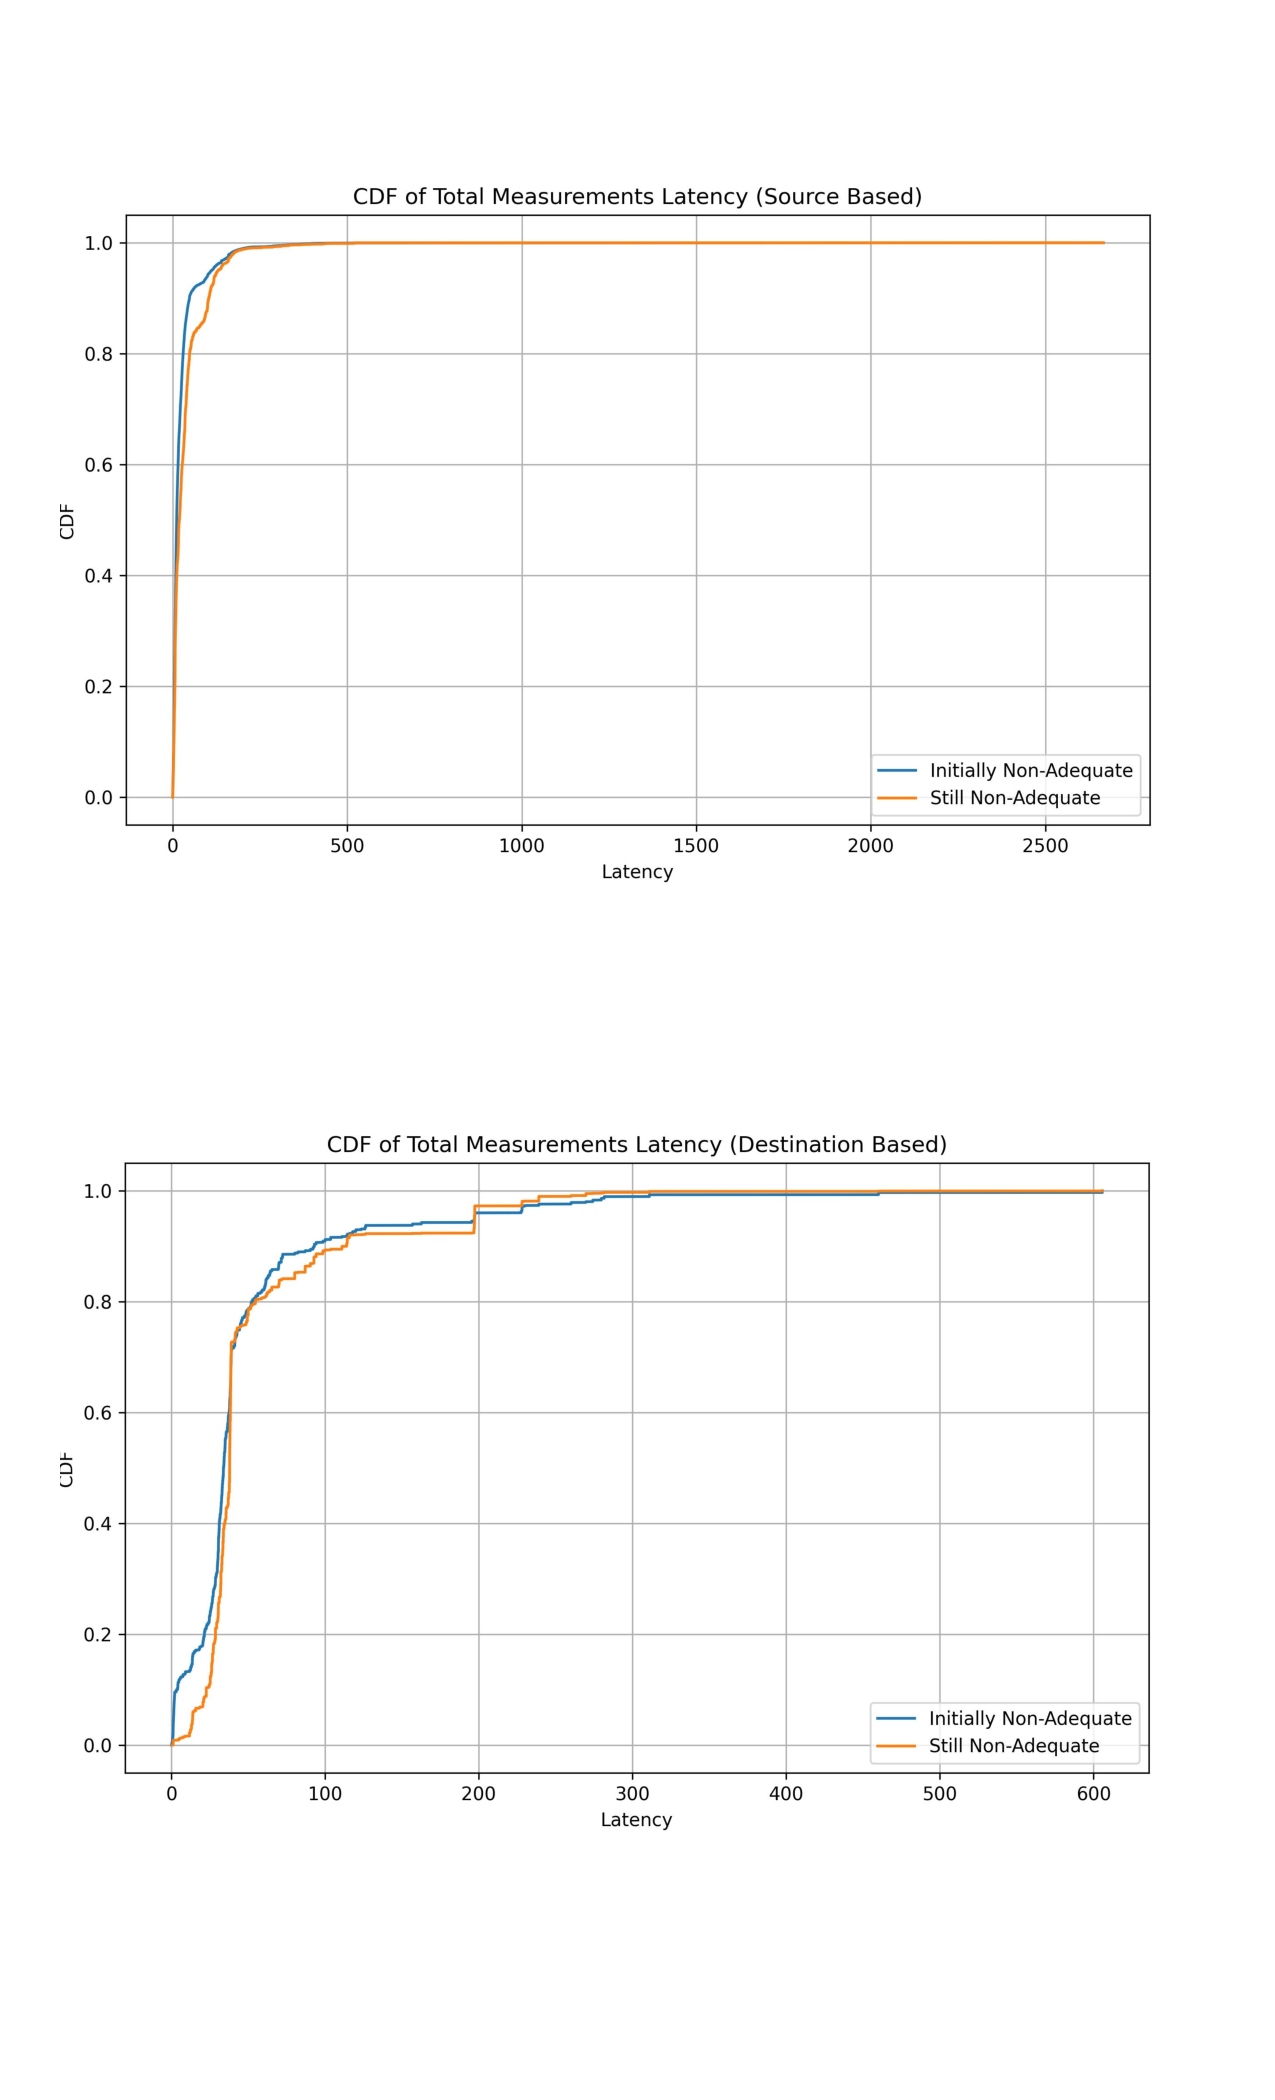
\includegraphics[width=.46\textwidth]{figures/Latencies.pdf}\\
    \caption{CDF of latency observed in source- and destination-based measurements.}
\label{fig:latencies}
\vspace{-4mm}
\end{figure}

\section*{B Ethics}
Our study does not collect personal information of any kind and does not
qualify as human subjects research. We collect data only from public, very popular web
sites and the resources that they load. We do not log in to any sites. We
use a separate browser that is routed through a proxy (not the user's own
browser). Thus we do not have access to any user's browsing history, data locally stored in
any user's device, any device/identifying information, nor any other private data.
The only exception is our limited experiment to confirm the accuracy of BrightData's
stated location of proxies; there, we only record the /24 subnet to which the device running the proxy
is connected.
In sum, our study is an investigation of the public web and does not pose significant ethical concerns.
The scale of our data collection, for all types of information we gather,
is unlikely to impact any services of the major websites we
study, and there are meaningful benefits in understanding compliance with online privacy regulations.
